\addchap{Regelmäßige Veranstaltungen auf dem Campus}

\minisec{Spieleabende}

Etwa einmal im Monat wird in der Fakultät vom FSR ein Spieleabend ausgerichtet. Start ist jeweils um 18:30 Uhr im Foyer. Dabei stellt der FSR sein umfangreiches Angebot an analogen Spielen zur Verfügung, sodass eine ganze Menge an Spielen schon von Haus aus da sind. Wollt ihr etwas spielen, was nicht da ist, bringt es am besten mit. Oft sind auch schnell Leute gefunden, die mal ein neues Spiel ausprobieren wollen.

Hin und wieder finden sich auch ein paar Leute, die an dem Abend ihre Notebooks mitbringen und eine kleine LAN-Party schmeißen oder ihre Spielekonsole mitbringen, um über einen der Beamer der Seminarräume mit anderen zusammen zu spielen.

Für Knabbereien und Getränke wird gesorgt, das \ascii{} hat in der Regel zu Spieleabenden geöffnet. Wenn das Wetter mitspielt, ist auch das \emph{Count Down}, ein Dresdner Studentenclub, zur Stelle und verkauft Heißes vom Grill sowie alkoholische Getränke.

Es lohnt sich also auf jeden Fall, vorbeizuschauen und bei einer Mate und einer frischen Bratwurst neue Leute kennenzulernen!

\minisec{Stammtische}

Wolltest du deine liebste Lehrperson schon immer mal etwas persönlicher kennenlernen? Der halbjährlich stattfindende Stammtisch bietet genau diese Möglichkeit. Hierbei setzt du dich völlig entspannt mit den beiden teilnehmenden Lehrpersonen in einem Studentenclub zusammen und kannst alle Fragen stellen, die dir schon lange oder vielleicht auch noch nicht so lange auf der Zunge brennen. Dies betrifft nicht nur fachliche, sondern vielmehr auch persönliche Fragen. Auch die teilnehmenden Lehrenden freuen sich hierbei über rege Beteiligung der Studierenden. Also komm doch vorbei.

\pagebreak

\
\thispagestyle{empty}
\AddToShipoutPicture*{\put(0,0){%
\parbox[b][\paperheight]{\paperwidth}{%
\vfill
\centering
\refstepcounter{dummy}
\label{spieleabendplakat}
\includegraphics[width=\dimen107,height=\dimen108,keepaspectratio]{img/spieleabend.png}%
\vfill
}}}

\pagebreak

\minisec{OUTPUT.DD}

Die OUTPUT.DD findet einmal im Jahr statt. Das erklärte Ziel dieser Veranstaltung ist es, der breiten Öffentlichkeit die Ergebnisse aus Lehre und Forschung zu präsentieren. Zu diesem Zwecke kommen einige große Unternehmen an unsere wunderschöne Fakultät, bauen ihren Stand auf und präsentieren sich. Für dich als Studierenden unserer Fakultät bietet dies die Chance, dich mit den Unternehmen der Region vertraut zu machen und in ungezwungenem Rahmen mit diesen ins Gespräch zu kommen. Dies kann ein gutes Sprungbrett für eventuelle Praktika oder Werkstudententätigkeiten sein. Des Weiteren gibt es oft kleine Gewinnspiele und Wettbewerbe mit Preisen für die Besucher. Ein Besuch dieser hervorragenden Veranstaltung sei dir also hiermit ans Herz gelegt. Es lohnt sich.

\begin{figure}[b!]
	\centering
  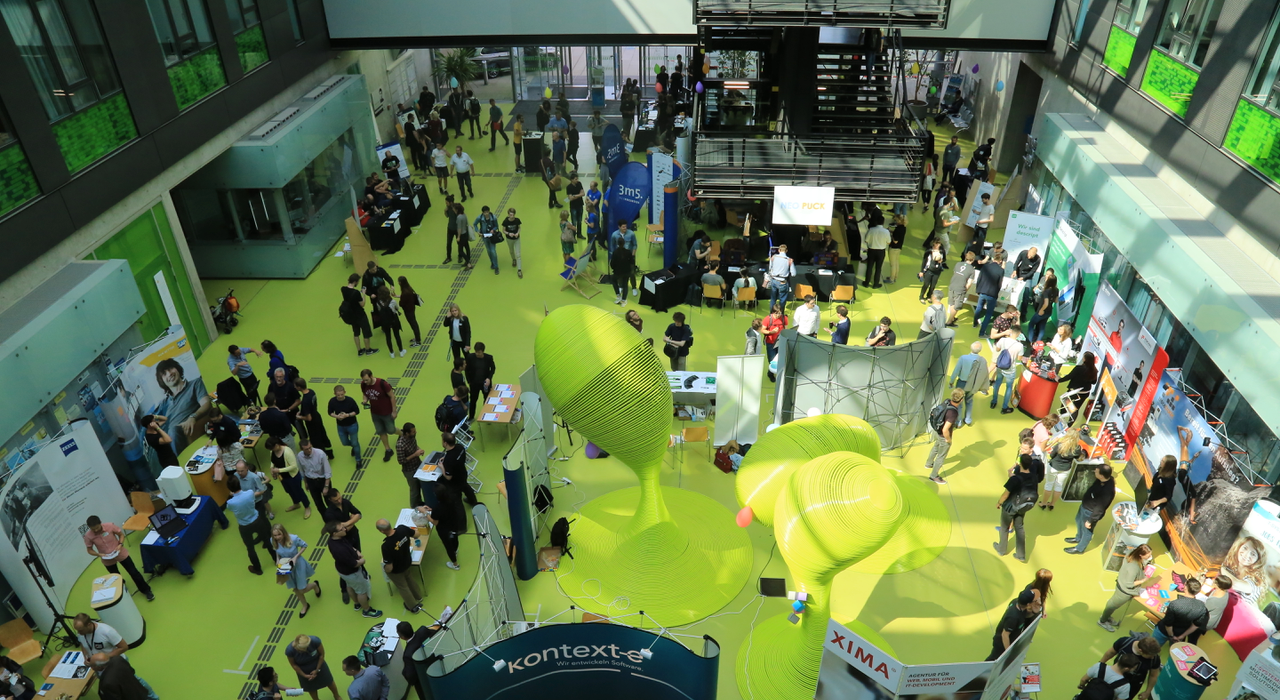
\includegraphics[width=\linewidth]{img/output}
  \caption*{\small \centering \textit{OUTPUT: Studierende stellen ihre Projekte und Firmen sich selbst vor. -- Foto: Lucas Vogel}}
\end{figure}%

\minisec{KIF}

Die Konferenz deutschsprachiger Informatik-Fachschaften (kurz KIF) findet halbjährlich statt. Hierbei wechselt die ausrichtende Stadt jedes Mal. Der FSR nimmt an jeder KIF mit einigen Personen teil und ist offen für neue Interessierte.

Im kommenden Jahr wird die Fachschaft Informatik der TU Dresden selber eine KIF im Zeitraum von Pfingsten, also vom 12.06.2019 bis zum 16.06.2019, ausrichten. Hierzu suchen wir immer helfende Hände für Planung und Durchführung, aber natürlich seid ihr auch herzlich eingeladen einfach nur teilzunehmen.

\pagebreak

Diese Veranstaltung ist eine großartige Chance sich mit den anderen Informatik Fachschaften aus Deutschland zu vernetzen und Einblicke in deren Studienalltag zu erlangen.

\minisec{ESE}

Die Erstsemestereinführung (kurz ESE) findet jedes Jahr Anfang Oktober statt um die neuen Studierenden unserer Fakultät zu begrüßen und sie in das Studium einzuführen. Veranstaltet wird diese vom FSR, der meist bereits kurz nach einer abgeschlossenen ESE damit beginnt die nächste ESE zu planen. Wie du dir sicherlich vorstellen kannst ist das ziemlich viel Arbeit, zumindest, wenn keiner dabei hilft.

Hier kommst du ins Spiel. Du fandest deine ESE super und möchtest dafür sorgen, dass auch alle weiteren Erstis eine super ESE haben? Oder fandest du deine ESE absolut schrecklich (wieso auch immer du das so sehen solltest) und hast tausend Ideen wie man es besser machen könnte? Wir als FSR laden dich herzlich dazu ein uns in Planung und Durchführung dieser wunderbaren Veranstaltung zu helfen und sie noch viel wunderbarer zu machen.

Wenn dich das Interesse gepackt hat, dann komm einfach bei uns im Büro vorbei und sag uns Bescheid.

\minisec{Studentenklub Count Down}

\begin{wrapfigure}{l}{3.25cm}%
  \vspace{-.5cm}
  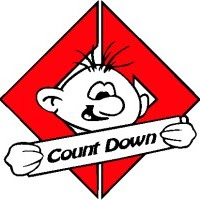
\includegraphics[width=\linewidth]{img/countdown}
  \vspace{-1cm}
\end{wrapfigure}

Wir, der Studentenklub IZ e.V., haben in den Tiefen des Wohnheims Güntzstraße 22, in der Dresdner Johannstadt unseren kleinen Studentenklub, das Count Down \link{https://www.countdown-dresden.de}.
IZ das steht für Informatikzentrum und tatsächlich sind wir der letzte Rest der Informatikfakultät in der Johannstadt, wo sie bis in die Mitte der 2000er ihre Heimat hatte.

Gemeinsam kochen wir, schauen Filme, zocken die Nächte durch, helfen uns gegenseitig durchs Studium oder treffen uns einfach nur so zu einer kleinen Runde Dart.
Außerdem gestalten wir zusammen als Mitglieder für euch den Rahmen unserer kleinen Bar in der Johannstadt.
Von der Auswahl der besten Biere und der leckersten Mate über die inhaltliche Gestaltung der verrücktesten Veranstaltungen und dem Mixen der absurdesten Cocktails an der Bar, bis hin zur Verschönerung des Clubs führen wir alles ehrenamtlich durch.
Dabei werden alle Entscheidungen demokratisch unter Einbezug der Kenntnis der erfahrenen Mitglieder und der frischen Ideen neuer Leute getroffen.

\pagebreak

Zu unseren derzeitigen Veranstaltungen gehören bspw. Spieleabende, verschiedene Metalpartys, der gemeinsame Erasmus-Länderabend mit der ESN-Initiative der TU-Dresden, Werewolf- oder Cocktailabende.

\begin{wrapfigure}{r}{3.25cm}%
  \vspace{-.5cm}
  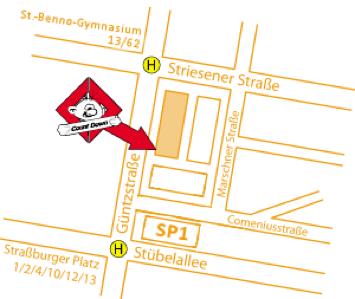
\includegraphics[width=\linewidth]{img/cd-anfahrt}
  \vspace{-1cm}
\end{wrapfigure}

Sind als nächstes auch deine tollen Ideen dabei?
Wir freuen uns immer über Nachwuchs und frische Ideen.
Komm bei uns vorbei und sprich uns an der Bar an, schreib uns eine E-Mail \link{mailto:cd@iz-ev.de} oder bei Facebook \link{https://www.facebook.com/countdowndd} und einer Mitgliedschaft steht nichts im Weg.
Auch die Arbeit hinter der Bar haben wir bisher noch jedem beibringen können.

\begin{itemize}
    \item[$\rhd$] \textbf{Öffnungszeiten:}
    \begin{itemize}[noitemsep]
        \item Mo \& Mi: 19:00 – 0:00
        \item Di: 20:00 – 1:00
        \item sowie ausgewählte Samstage
    \end{itemize}
\end{itemize}

\begin{figure}[b!]
  \centering
  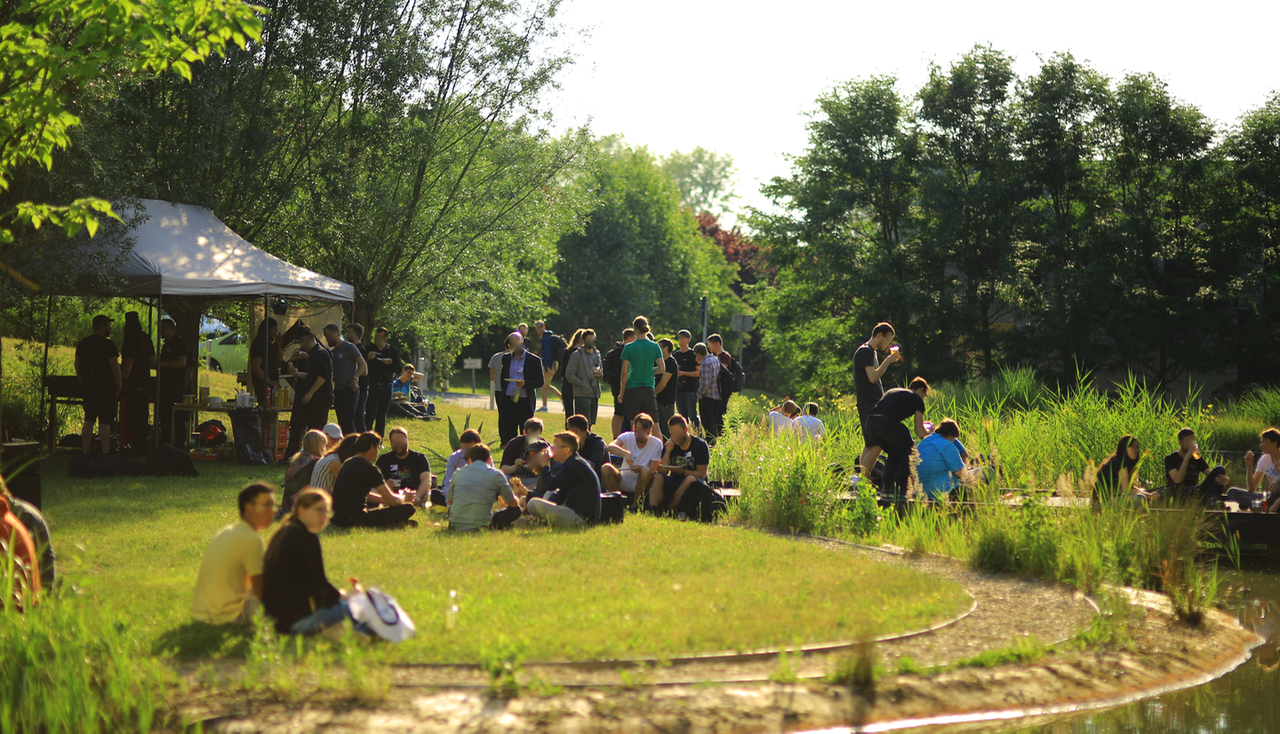
\includegraphics[width=\linewidth]{img/output_pond}
  \caption*{\small \centering \textit{Zur OUTPUT wird der Teich zur Lounge -- mit Musik, Freibier und frischem Essen vom Grill. Foto: Lucas Vogel}}
\end{figure}


\minisec{Allgemein}

Alle hier genannten Veranstaltungen werden, kurz bevor sie tatsächlich stattfinden, auch nochmal auf sozialen Medien und über Plakate in der Fakultät beworben mit den jeweiligen detaillierten Informationen.
